\documentclass[hyperref={pdfpagelabels=false}]{beamer}

\usepackage{xeCJK}
\setCJKmainfont[AutoFakeSlant=0.25]{Noto Sans Mono CJK SC}
\setCJKsansfont[AutoFakeSlant=0.25]{Noto Sans Mono CJK SC}
\setCJKmonofont[AutoFakeSlant=0.25]{Noto Sans Mono CJK SC}

\setbeamertemplate{bibliography item}[text]

\usepackage{python}
\usepackage{lmodern}
\usepackage{datetime}
\usetheme{Madrid}
\usecolortheme{dolphin}
\title{科技论文写作文献检索}  
\subtitle{联邦学习中的通信优化}
\author{叶茂青 \and 王珺} 

\newdate{date}{12}{06}{2020}
\date{\displaydate{date}}

\begin{document}
\begin{frame}
\titlepage
\end{frame} 

\begin{frame}
	\frametitle{总览}
	\tableofcontents
\end{frame} 

\section{介绍}
\begin{frame}
	\tableofcontents[currentsection]
\end{frame} 

\begin{frame}
	\frametitle{联邦学习的定义}
	\begin{itemize}
		\item 联邦学习的数学模型被McMahan et al.\cite{mcmahan2016communication}定义为$$\min _{w} F(w), \text { where } F(w):=\sum_{k=1}^{m} p_{k} F_{k}(w)$$
		\item 通俗来说,就是多个客户端通过中心服务器的协调合作解决一个机器学习问题
	\end{itemize}
	\begin{figure}
		\centering
		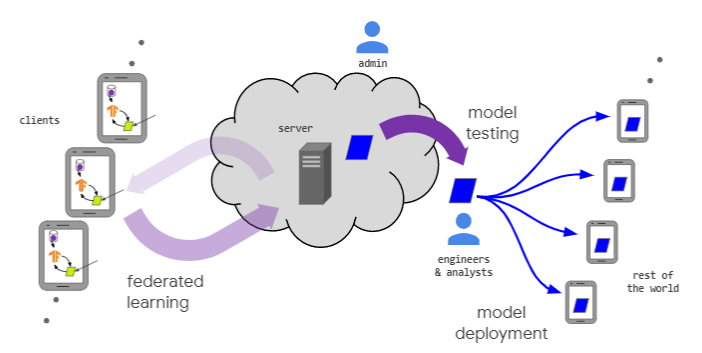
\includegraphics[width=.6\textwidth]{./figure/1.png}
		\caption{The lifecycle of an FL-trained model.\cite{kairouz2019advances}}
	\end{figure}
\end{frame}


\begin{frame}
	\frametitle{联邦学习的特点}
	\begin{itemize}
		\item<+-> 客户端数据保存在本地,不会上传给服务器
		\item<+-> 数据不满足IID(独立同分布)假设
		\item<+-> 客户端的处理能力,带宽是有限的,且不一定可靠
	\end{itemize}
\end{frame}

\begin{frame}
	\frametitle{联邦学习的分类}
	\begin{itemize}
		\item 横向联邦学习
		\item 纵向联邦学习
		\item 联邦迁移学习
	\end{itemize}
\end{frame}

\begin{frame}
	\frametitle{横向联邦学习}
	\begin{block}{}
		适用于特征重叠多,但用户重叠少的情况,比如不同地区之间的银行、医院,参与的设备数一般较少,且客户端基本可保持稳定
	\end{block}
	\begin{figure}
		\centering
		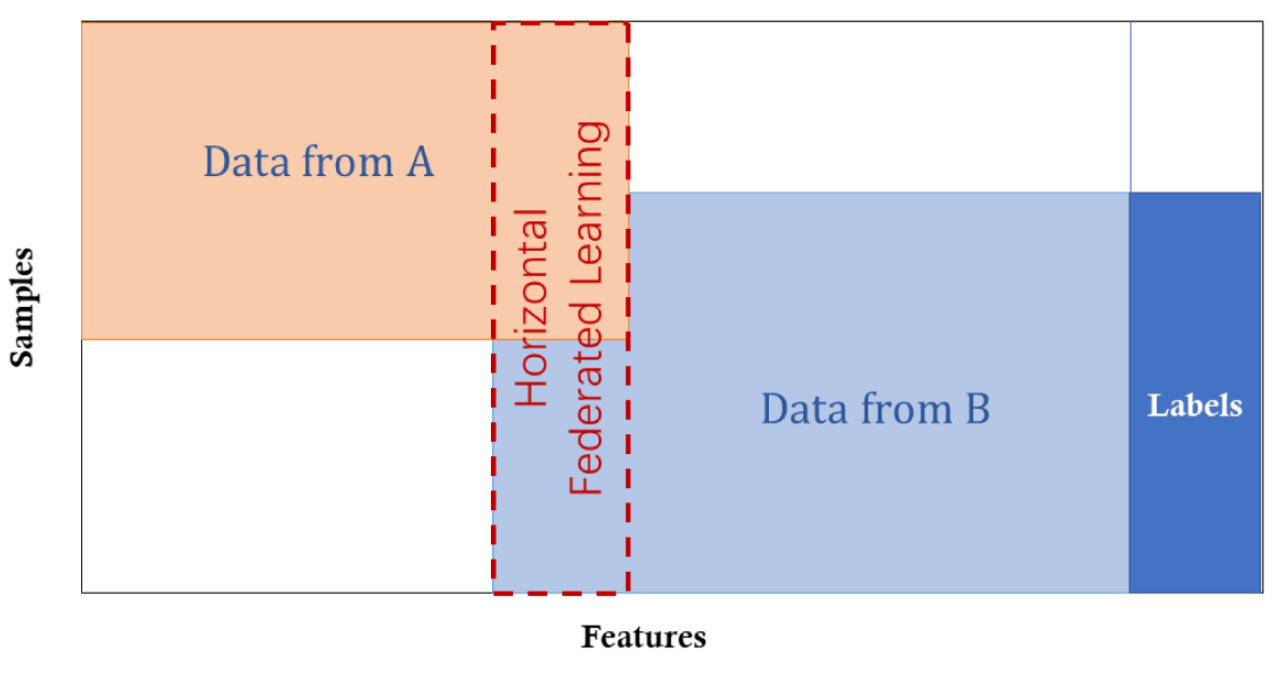
\includegraphics[width=.6\textwidth]{./figure/hor-fl.png}
		\caption{Horizontal Federated Learning\cite{yang2019federated}}
	\end{figure}
\end{frame}

\begin{frame}
	\frametitle{纵向联邦学习}
	\begin{block}{}
		适用于特征重叠少,但用户重叠多的情况,比如使用同一个app的用户,参与的设备数数量级庞大,客户端不可靠,不能保证稳定在线,且有可能存在攻击者
	\end{block}
	\begin{figure}
		\centering
		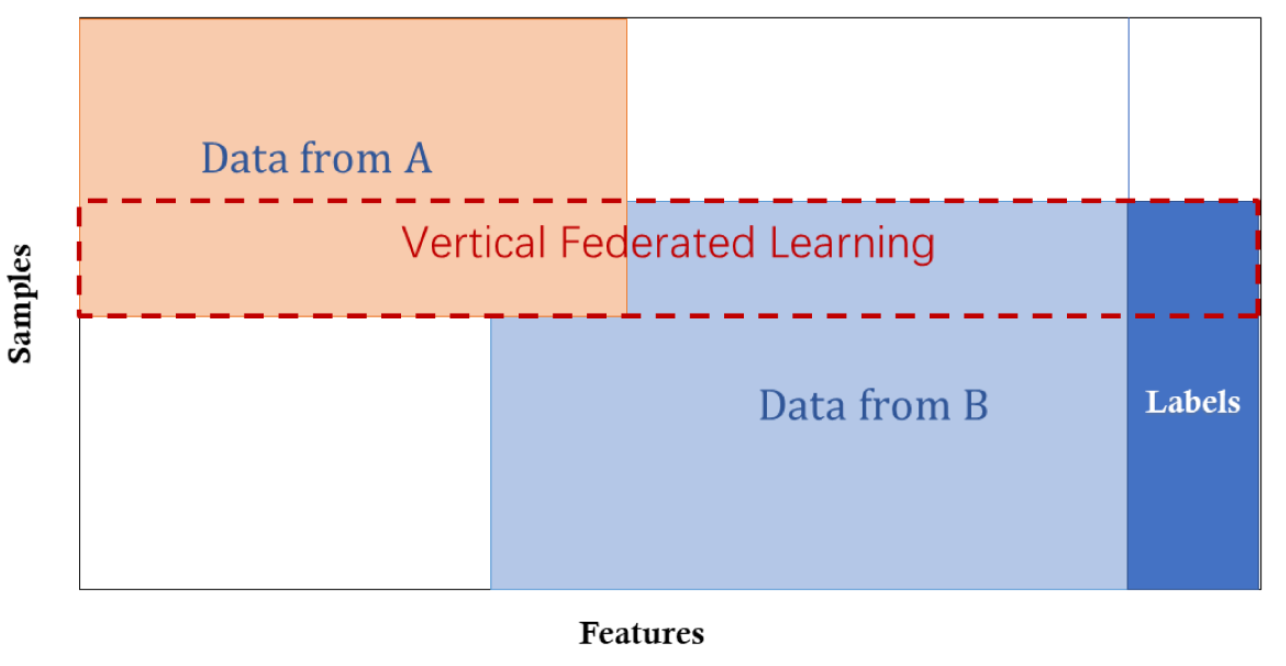
\includegraphics[width=.6\textwidth]{./figure/ver-fl.png}
		\caption{Vertical Federated Learning\cite{yang2019federated}}
	\end{figure}
\end{frame}

\begin{frame}
	\frametitle{联邦迁移学习}
	\begin{block}{}
		对于特征和用户重叠都较少的状况,比如不同领域的不同公司,需要利用迁移学习来提升模型的效果
	\end{block}
	\begin{figure}
		\centering
		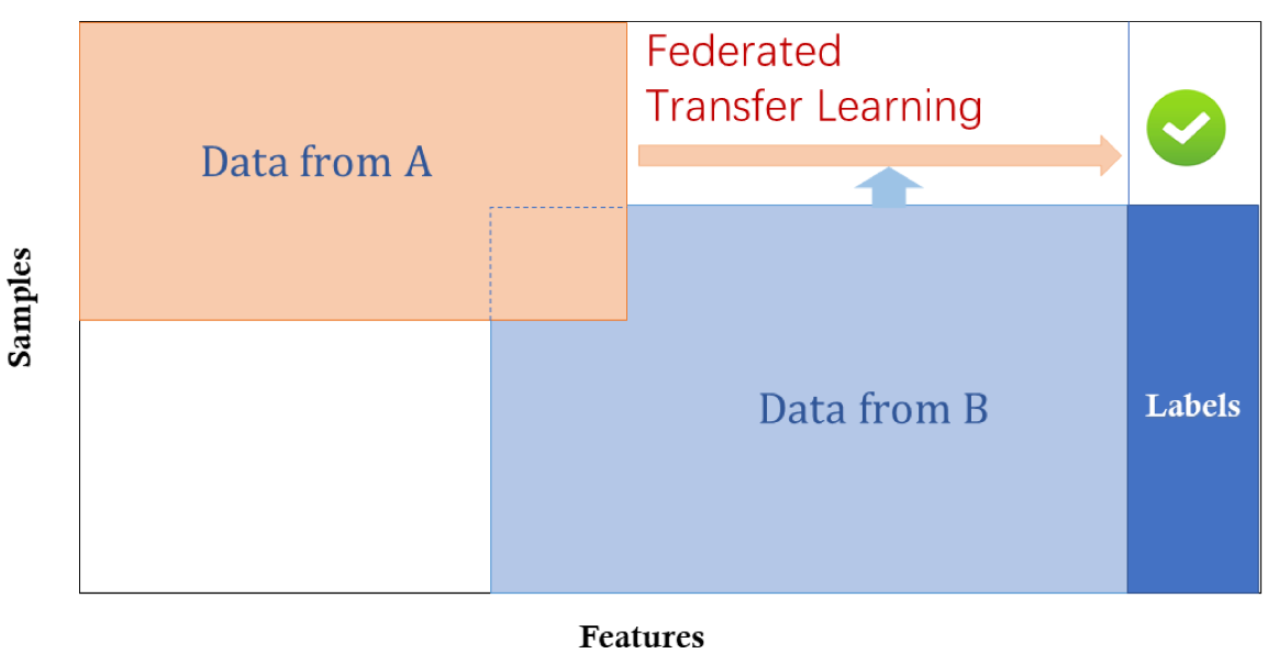
\includegraphics[width=.6\textwidth]{./figure/fl-tran.png}
		\caption{Federated Transfer Learning\cite{yang2019federated}}
	\end{figure}
\end{frame}

\section{文献搜索}
\begin{frame}
	\tableofcontents[currentsection]
\end{frame} 
\begin{frame}
	\frametitle{寻找综述论文}
	\begin{figure}
		\centering
		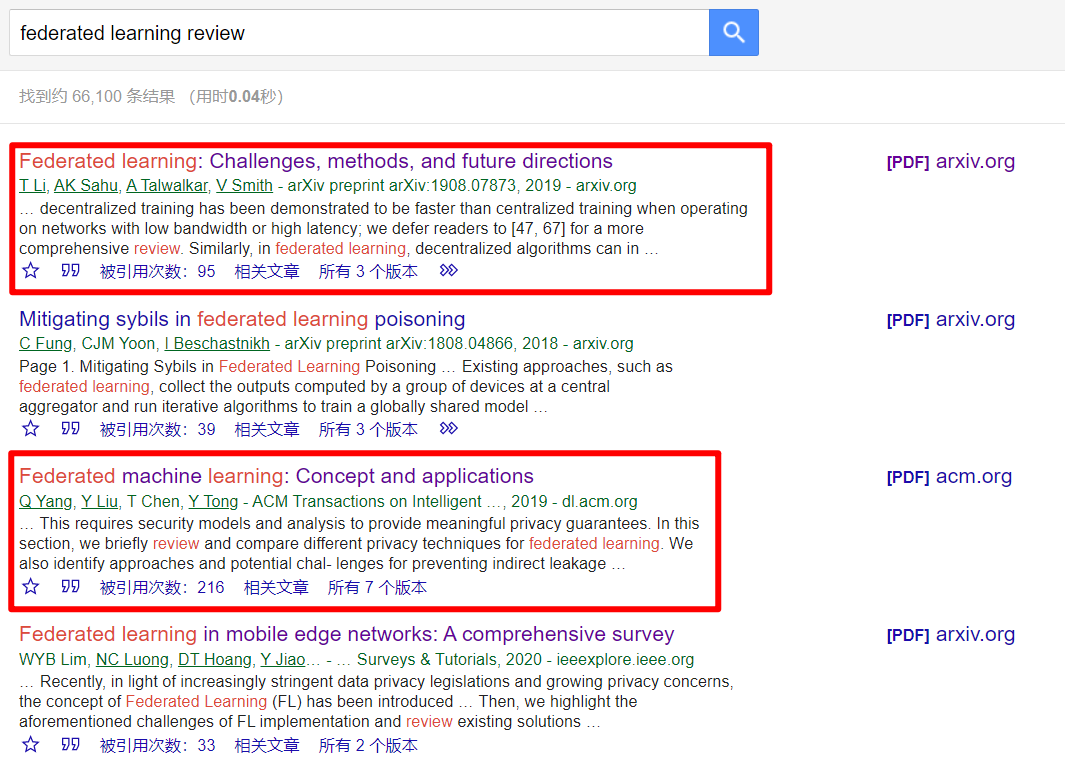
\includegraphics[height=0.8\textheight]{./figure/2.png}
	\end{figure}
\end{frame}

\begin{frame}
	\frametitle{寻找综述论文}
	\begin{figure}
		\centering
		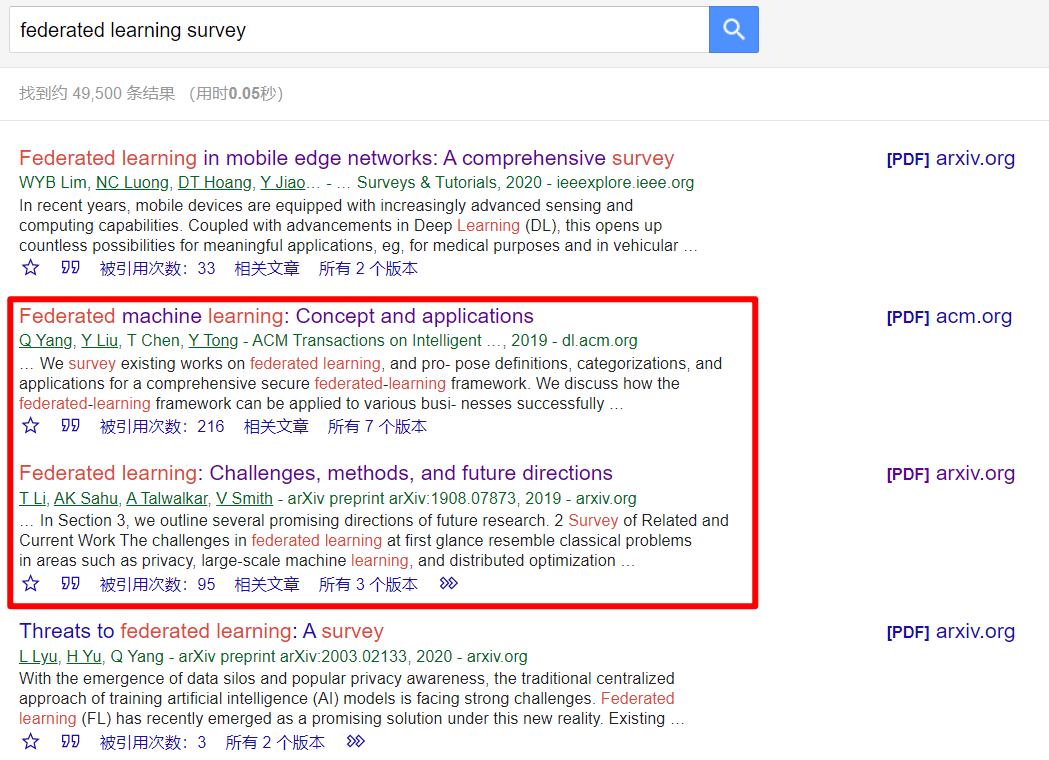
\includegraphics[height=0.8\textheight]{./figure/3.png}
	\end{figure}
\end{frame}

\begin{frame}
	\frametitle{了解定义及相关问题}
	\begin{itemize}
		\item 什么是联邦学习?
		\item 联邦学习有哪些核心问题?
		\item 对于这些核心问题,解决方案有哪些?研究方向是什么?
	\end{itemize}
\end{frame}

\begin{frame}
	\frametitle{整理脉络}
	\begin{figure}
		\centering
		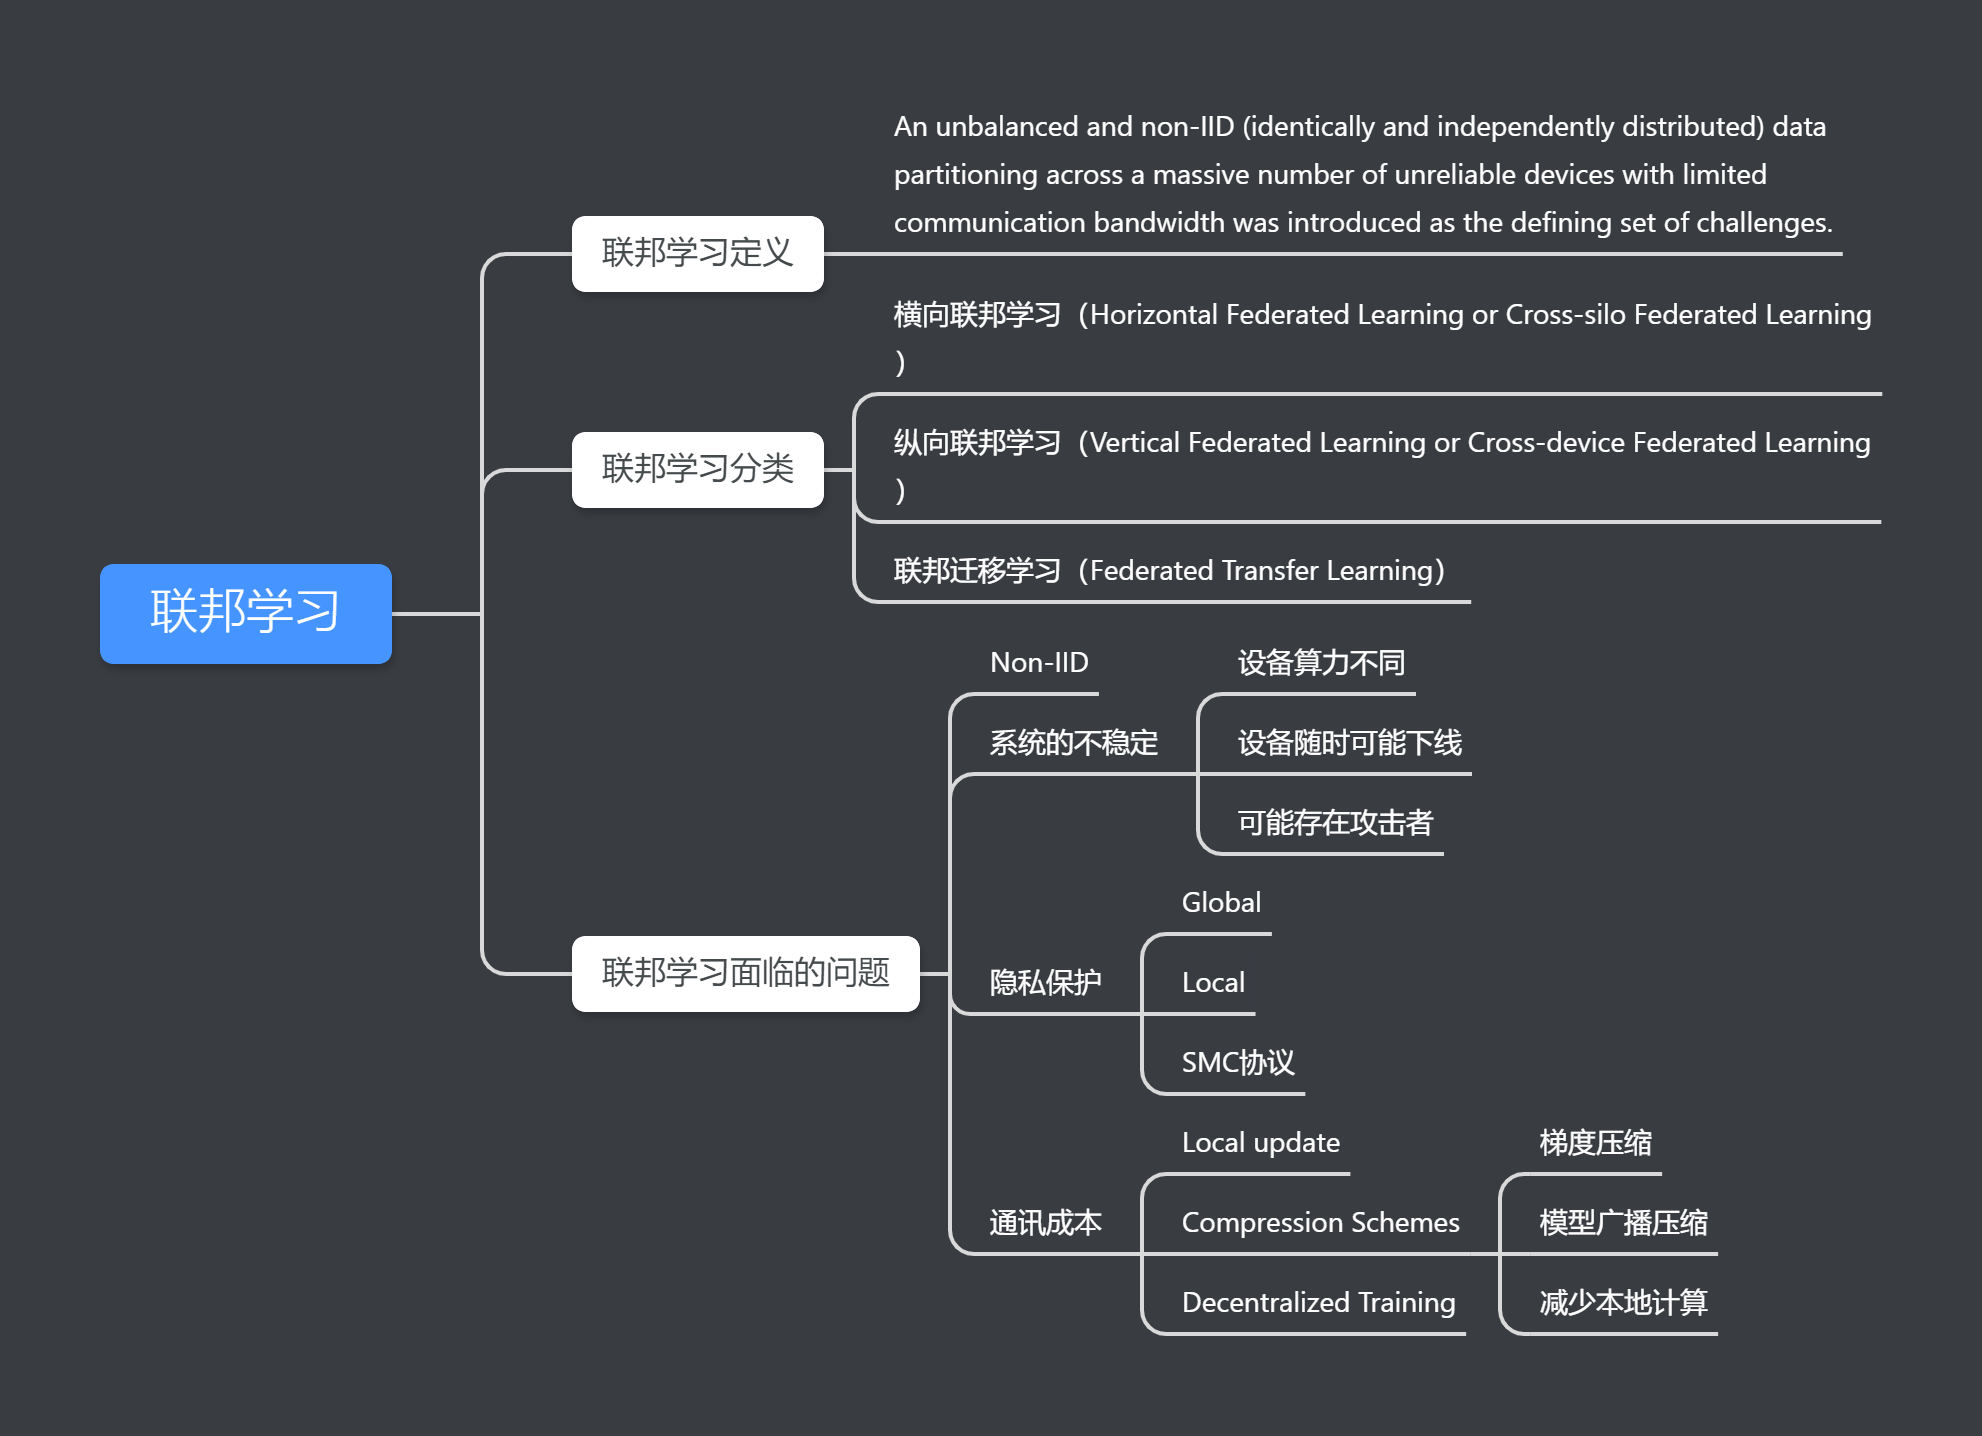
\includegraphics[height=0.8\textheight]{./figure/mubu.png}
	\end{figure}
\end{frame}

\begin{frame}
	\frametitle{细化领域}
	联邦学习中的通信优化方法主要有三类,核心思想在于减少通信的次数或降低通信所耗的带宽
	\begin{itemize}
		\item Local update
		\item Compression Schemes
		\item Decentralized Training
	\end{itemize}
\end{frame}

\begin{frame}
	\frametitle{细化领域}
	通过相关论文的Related Work再寻找细化领域的相关研究
	\begin{figure}
		\centering
		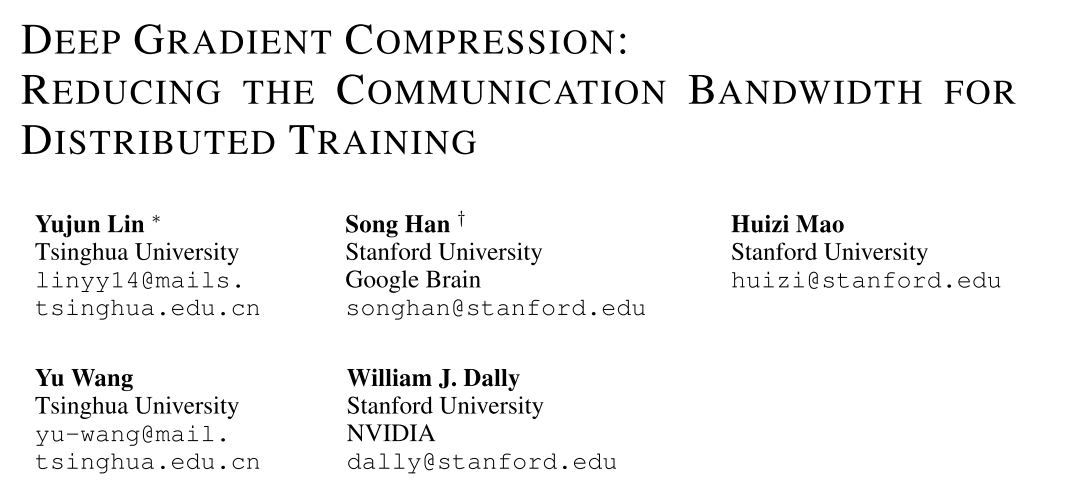
\includegraphics[height=0.6\textheight]{./figure/4.png}
	\end{figure}
\end{frame}

\begin{frame}
	\frametitle{细化领域}
	通过相关论文的Related Work再寻找细化领域的相关研究
	\begin{figure}
		\centering
		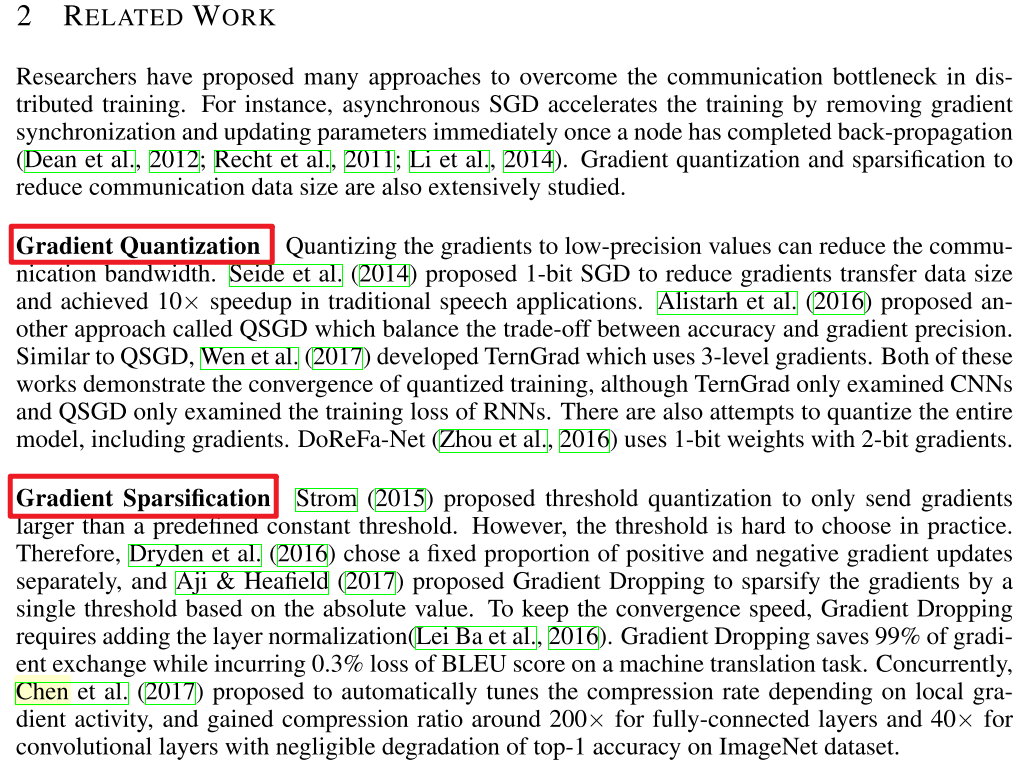
\includegraphics[height=0.8\textheight]{./figure/5.png}
	\end{figure}
\end{frame}

\section{文献阅读}
\begin{frame}
	\tableofcontents[currentsection]
\end{frame} 


\begin{frame}
	\frametitle{文献阅读}
	按使用的方法整理各类文献,记下文献提出的算法,使用的模型
	\begin{figure}
		\centering
		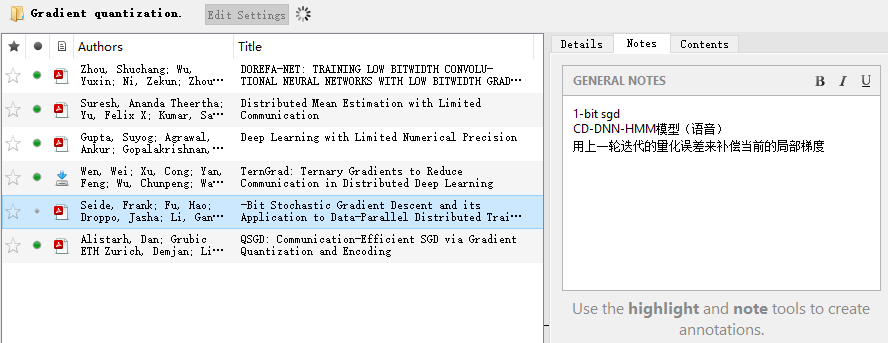
\includegraphics[height=0.5\textheight]{./figure/6.png}
	\end{figure}
\end{frame}


\begin{frame}[allowframebreaks]
	\frametitle{References}
	\bibliographystyle{IEEEtran}
	\bibliography{ppt.bib}
\end{frame}

\begin{frame}{}
	\centering \Huge
	\emph{Thank You!}
\end{frame} 

\end{document}

